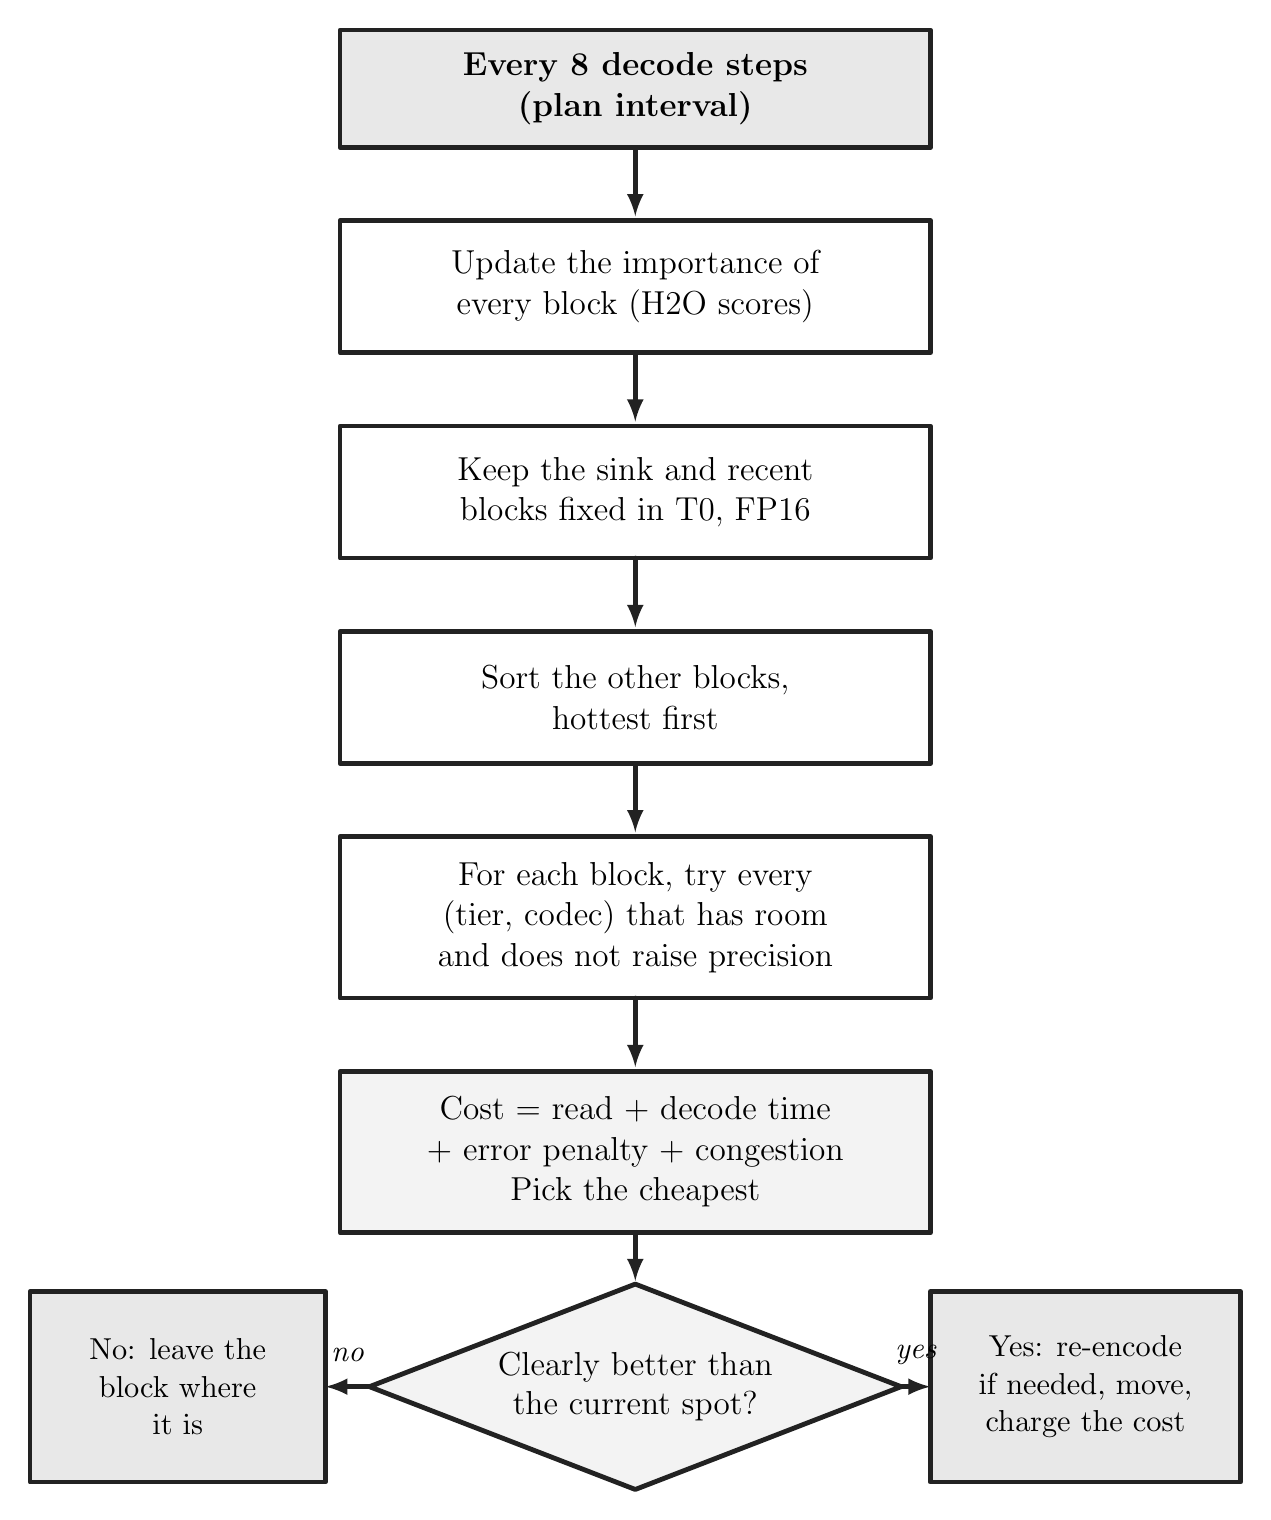
\begin{tikzpicture}[line cap=round,line join=round]
\draw[line width=1.74pt,draw={rgb,255:red,34;green,34;blue,34},fill={rgb,255:red,232;green,232;blue,232}] (1.624in,6.893in) rectangle (4.576in,7.480in);
\draw[line width=1.74pt,draw={rgb,255:red,34;green,34;blue,34},fill={rgb,255:red,255;green,255;blue,255}] (1.624in,5.867in) rectangle (4.576in,6.527in);
\draw[line width=1.74pt,draw={rgb,255:red,34;green,34;blue,34},fill={rgb,255:red,255;green,255;blue,255}] (1.624in,4.840in) rectangle (4.576in,5.500in);
\draw[line width=1.74pt,draw={rgb,255:red,34;green,34;blue,34},fill={rgb,255:red,255;green,255;blue,255}] (1.624in,3.813in) rectangle (4.576in,4.473in);
\draw[line width=1.74pt,draw={rgb,255:red,34;green,34;blue,34},fill={rgb,255:red,255;green,255;blue,255}] (1.624in,2.640in) rectangle (4.576in,3.447in);
\draw[line width=1.74pt,draw={rgb,255:red,34;green,34;blue,34},fill={rgb,255:red,243;green,243;blue,243}] (1.624in,1.467in) rectangle (4.576in,2.273in);
\draw[line width=1.74pt,draw={rgb,255:red,34;green,34;blue,34},fill={rgb,255:red,243;green,243;blue,243}] (3.100in,1.210in) -- (4.429in,0.697in) -- (3.100in,0.183in) -- (1.771in,0.697in) -- cycle;
\draw[line width=1.74pt,draw={rgb,255:red,34;green,34;blue,34},fill={rgb,255:red,232;green,232;blue,232}] (4.576in,0.220in) rectangle (6.126in,1.173in);
\draw[line width=1.74pt,draw={rgb,255:red,34;green,34;blue,34},fill={rgb,255:red,232;green,232;blue,232}] (0.074in,0.220in) rectangle (1.550in,1.173in);
\node[align=center,text={rgb,255:red,0;green,0;blue,0},font=\fontsize{12.4pt}{14.6pt}\selectfont\bfseries,inner sep=0pt] at (3.100in,7.187in) {Every 8 decode steps \\ (plan interval)};
\node[align=center,text={rgb,255:red,0;green,0;blue,0},font=\fontsize{12.4pt}{14.6pt}\selectfont,inner sep=0pt] at (3.100in,6.197in) {Update the importance of \\ every block (H2O scores)};
\node[align=center,text={rgb,255:red,0;green,0;blue,0},font=\fontsize{12.4pt}{14.6pt}\selectfont,inner sep=0pt] at (3.100in,5.170in) {Keep the sink and recent \\ blocks fixed in T0, FP16};
\node[align=center,text={rgb,255:red,0;green,0;blue,0},font=\fontsize{12.4pt}{14.6pt}\selectfont,inner sep=0pt] at (3.100in,4.143in) {Sort the other blocks, \\ hottest first};
\node[align=center,text={rgb,255:red,0;green,0;blue,0},font=\fontsize{12.4pt}{14.6pt}\selectfont,inner sep=0pt] at (3.100in,3.043in) {For each block, try every \\ (tier, codec) that has room \\ and does not raise precision};
\node[align=center,text={rgb,255:red,0;green,0;blue,0},font=\fontsize{12.4pt}{14.6pt}\selectfont,inner sep=0pt] at (3.100in,1.870in) {Cost = read + decode time \\ + error penalty + congestion \\ Pick the cheapest};
\node[align=center,text={rgb,255:red,0;green,0;blue,0},font=\fontsize{11.9pt}{14.0pt}\selectfont,inner sep=0pt] at (3.100in,0.697in) {Clearly better than \\ the current spot?};
\draw[-latex,line width=1.74pt,draw={rgb,255:red,34;green,34;blue,34}] (3.100in,6.893in) -- (3.100in,6.549in);
\draw[-latex,line width=1.74pt,draw={rgb,255:red,34;green,34;blue,34}] (3.100in,5.867in) -- (3.100in,5.522in);
\draw[-latex,line width=1.74pt,draw={rgb,255:red,34;green,34;blue,34}] (3.100in,4.840in) -- (3.100in,4.495in);
\draw[-latex,line width=1.74pt,draw={rgb,255:red,34;green,34;blue,34}] (3.100in,3.813in) -- (3.100in,3.469in);
\draw[-latex,line width=1.74pt,draw={rgb,255:red,34;green,34;blue,34}] (3.100in,2.640in) -- (3.100in,2.295in);
\draw[-latex,line width=1.74pt,draw={rgb,255:red,34;green,34;blue,34}] (3.100in,1.467in) -- (3.100in,1.225in);
\node[align=center,text={rgb,255:red,0;green,0;blue,0},font=\fontsize{11.4pt}{13.5pt}\selectfont,inner sep=0pt] at (5.351in,0.697in) {Yes: re-encode \\ if needed, move, \\ charge the cost};
\node[align=center,text={rgb,255:red,0;green,0;blue,0},font=\fontsize{11.4pt}{13.5pt}\selectfont,inner sep=0pt] at (0.812in,0.697in) {No: leave the \\ block where \\ it is};
\draw[-latex,line width=1.74pt,draw={rgb,255:red,34;green,34;blue,34}] (4.429in,0.697in) -- (4.576in,0.697in);
\node[align=center,text={rgb,255:red,0;green,0;blue,0},font=\fontsize{11.4pt}{13.5pt}\selectfont\itshape,inner sep=0pt] at (4.502in,0.858in) {yes};
\draw[-latex,line width=1.74pt,draw={rgb,255:red,34;green,34;blue,34}] (1.771in,0.697in) -- (1.550in,0.697in);
\node[align=center,text={rgb,255:red,0;green,0;blue,0},font=\fontsize{11.4pt}{13.5pt}\selectfont\itshape,inner sep=0pt] at (1.661in,0.858in) {no};
\end{tikzpicture}
